\documentclass{boi2014-lt}

\usepackage{enumitem}
\usepackage{wrapfig}
\usepackage{mathtools}
\usepackage{tikz}

\renewcommand{\DayNum}{1}
\renewcommand{\TaskCode}{coprobber}
\renewcommand{\TaskName}{Policininkas ir plėšikas}

\renewcommand{\labelitemii}{$\circ$}
\newcommand{\constant}[1]{{\tt #1}}

\begin{document}
    \begin{wrapfigure}[11]{r}{6cm}
		\includegraphics[width=6cm]{\TaskCode.jpeg}
	\end{wrapfigure}

	Bitangoje nusikalstamumo lygis muša visų laikų rekordus. Be kitų
	nusikaltimų, kasdien vyksta apiplėšimai. Kaskart įvykus nusikaltimui vienišam
	policininkui tenka gaudyti plėšiką, sprunkantį siaurais skersgatviais, kurie
	jungia įvairius miesto užkampius. Deja, dažniausiai plėšikai
	pasprunka nuo persekiotojų, kadangi jie pažįsta miestą žymiai geriau už
	pareigūnus.

	Bitangos miesto policijos departamentas (BMPD) organizuoja aukščiausio
	lygio susitikimą dėl nusikalstamumo mažinimo. Viena jų iniciatyvų yra
	persekioti plėšikus į pagalbą pasitelkiant kompiuterį. Tam BMPD sudarė
	tikslų miesto žemėlapį. Dabar jiems reikia programinės įrangos, kuri
	sukurtų persekiojimo strategijas.

	Vieną plėšiką persekiojančio vieno policininko uždavinys modeliuojamas taip:
	\begin{enumerate}
		\item Policijos pareigūnas pasirenka vieną užkampį ir ima jame
			patruliuoti.
		\item Tada plėšikas pasirenka užkampį apiplėšimui (jis žino, kur yra
			pareigūnas). Daroma prielaida, jog nuo šios akimirkos ir
			pareigūnas, ir plėšikas žino vienas kito buvimo vietą.
		\item Policijos pareigūno ėjimo metu jis nukeliauja į gretimą užkampį
			(t.~y. užkampį, kurį su dabartiniu užkampiu jungia skersgatvis)
			arba laukia (t.~y. nepajuda niekur).
		\item Plėšikas ėjimo metu nukeliauja į gretimą užkampį. Atkreipkite
			dėmesį, jog priešingai negu policininkas, plėšikas laukti negali.
			Instinktas jiems liepia nepaliaujamai bėgti.
		\item Policijos pareigūnas ir plėšikas vienas po kito atlieka ėjimus
			(pirmas eina pareigūnas) tol, kol kuri nors iš šių sąlygų tampa
			patenkinta:
			\begin{enumerate}
				\item situacija pasikartoja (situacija yra apibrėžta abiejų
					dalyvių pozicijomis bei kieno eilė yra daryti ėjimą).
					Tai reiškia, jog plėšikas sugebės išvengti policijos
					kiek norima ilgai, taigi plėšikas pasprunka;
				\item policijos pareigūnas ir plėšikas susitinka tame pačiame
					užkampyje po bet kurio iš jų ėjimo. Šiuo atveju policijos
					pareigūnas pagauna plėšiką.
			\end{enumerate}
	\end{enumerate}

    \Task
	Turite parašyti programą, kuri pagal duotą miesto žemėlapį nustatytų,
	ar įmanoma pagauti plėšiką, ir jeigu tai yra įmanoma, pagautų jį
	darydama ėjimus už policijos pareigūną.

	Jūsų programa turi daryti prielaidą, jog plėšikas juda optimaliai.

    \Implementation
    Turite realizuoti dvi funkcijas:
    \begin{itemize}
        \item \method{start(N, A)}, kuri priima šiuos argumentus:
            \begin{itemize}
                \item $N$ -- užkampių skaičius (užkampiai yra sunumeruoti
                    nuo $0$ iki $N-1$);
                \item $A$ -- dvimatis masyvas, apibūdinantis skersgatvius:
                    kiekvienam $0 \le i, j \le N-1$,
                    $$
                        A[i, j] \text{ yra }
                        \begin{dcases*}
                            \texttt{false} & jeigu $i$ ir $j$ nejungia
                                             skersgatvis
                                \\
                            \texttt{true} & jeigu $i$ ir $j$ jungia skersgatvis
                        \end{dcases*}
                    $$
                    Visi skersgatviai bus dvikrypčiai (t.~y. $A[i, j] = A[j, i]$
                    su kiekviena galima $i$ ir $j$ reikšme) ir nebus jokių
                    skersgatvių, jungiančių užkampį su juo pačiu (t.~y. $A[i, i]$
                    bus \texttt{false} kiekvienam galimam $i$). Be to, galite
                    daryti prielaidą, jog judant skersgatviais visada bus įmanoma
                    iš bet kurio užkampio pasieki bet kurį kitą.
            \end{itemize}

		Jeigu duotame žemėlapyje įmanoma pagauti plėšiką, funkcija \method{start}
		turi grąžinti užkampio, kuriame policijos pareigūnas pasirenka
		patruliuoti, numerį. Priešingu atveju, ji turi gražinti $-1$.

		\item \method{nextMove(R)}, priimanti vieną argumentą $R$ --- užkampio,
			kuriame dabar yra plėšikas, numerį. Ji turi grąžinti užkampio,
			kuriame policijos pareigūnas bus po savo ėjimo, numerį.
    \end{itemize}

    Funkcija \method{start} bus iškviesta lygiai vieną kartą, prieš bet kurį
    funkcijos \method{nextMove} iškvietimą. Jeigu \method{start} grąžina
    $-1$, funkcija \method{nextMove} nebus iškviesta. Priešingu atveju,
	\method{nextMove} bus pakartotinai kviečiama tol, kol baigsis persekiojimas.
    Tiksliau, programa baigs darbą atsiradus kuriai nors iš šių sąlygų:
    \begin{itemize}
        \item \method{nextMove} grąžina neleistiną ėjimą;
        \item situacija pasikartoja;
        \item plėšikas pagaunamas.
    \end{itemize}

    \Example
    \begin{wrapfigure}[4]{r}{2cm}
        \vspace{-0.5cm}
        \centering
        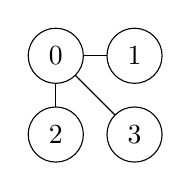
\begin{tikzpicture}
        \draw (0,1) -- (0,0);
        \draw (0,1) -- (1,0);
        \draw (0,1) -- (1,1);
        \foreach \x in {0,1} \foreach \y in {0,1}
            \draw (\x,\y) node[circle,draw,fill=white,inner sep=0,minimum size=0.7cm] {\pgfmathparse{int(2-2*\y+\x)}\pgfmathresult};
        \end{tikzpicture}
    \end{wrapfigure}
	Pažiūrėkime į dešinėje pavaizduotą pavyzdį. Šiuo atveju, bet kuris užkampis
	policijos pareigūnui yra gera pradinė pozicija. Jeigu jis pradės užkampyje
	Nr. 0, jis gali laukti savo pirmą ėjimą ir plėšikas pats pas jį atbėgs.
	Kitu atveju, jei jis pradės kuriame nors kitame užkampyje, jis gali laukti,
	kol plėšikas atsidurs užkampyje Nr. 0, ir tada nueiti į jį.
    
    Funkcijų vykdymo eiga galėtų būti tokia:

    \begin{tabular}{|l|c|}
        \hline
            {\bf Funkcijos kvietimas} & {\bf Grąžina} \\
        \hline
            \method{start(4, [[0, 1, 1, 1], [1, 0, 0, 0], [1, 0, 0, 0], [1, 0, 0, 0]])} &
            \constant{3} \\
        \hline
            \method{nextMove(1)} & \constant{3} \\
        \hline
            \method{nextMove(0)} & \constant{0} \\
        \hline
    \end{tabular}

	Pastaba: \method{start} kvietime trumpumo vardan \constant{false} žymima
	\constant{0} ir \constant{true} žymima \constant{1}.

    \Scoring
    
    \begin{description}
        \item[Dalinė užduotis Nr. 1 (16 taškų):] $2 \le N \le 500$.
        Kiekvieną užkampių porą jungs lygiai viena skersgatvių seka.
        \item[Dalinė užduotis Nr. 2 (14 taškų):] $2 \le N \le 500$.
			Užkampių ir skersgatvių tinklas suformuos tinklelį primenančią struktūrą.
			Tinklelis turės bent dvi eilutes ir stulpelius, o užkampiai bus
			sunumeruoti tokia tvarka, kaip pavaizduota žemiau.
        \begin{figure}[h!]
           \centering
           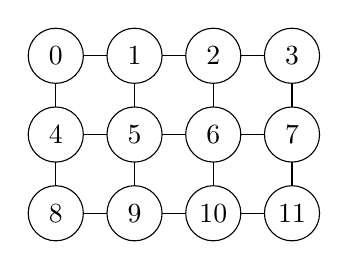
\begin{tikzpicture}
            \draw (0,0) grid (3,2);
            \foreach \x in {0,1,2,3} \foreach \y in {0,1,2}
                \draw (\x,\y) node[circle,draw,fill=white,inner sep=0,minimum size=0.7cm] {\pgfmathparse{int(8-4*\y+\x)}\pgfmathresult};
           \end{tikzpicture}
        \end{figure}
        \item[Dalinė užduotis Nr. 3 (30 taškų):] $2 \le N \le 100$.
        \item[Dalinė užduotis Nr. 4 (40 taškų):] $2 \le N \le 500$.
    \end{description}
    
    Jūsų sprendimas turėtų patenkinti du reikalavimus:
    \begin{enumerate}
    	\item teisingai nustatyti, ar policininkas gali pagauti plėšiką;
		\item sėkmingai sučiupti plėšiką darydama ėjimus už policijos
			pareigūną, jeigu įmanoma tai padaryti.
    \end{enumerate}
    
	Dalinėse užduotyse Nr. 1 ir Nr. 2 sprendimas surinks taškus tik tokiu
	atveju, jei patenkins abu reikalavimus.
	Dalinėse užduotyse Nr. 3 ir Nr. 4, sprendimai, kurie patenkina tik pirmą
	reikalavimą, surinks 30\% dalinės užduoties taškų.
	Jeigu jūsų sprendimas siekia tik dalinių taškų, galite nutraukti programos
	vykdymą atlikdami bet kokį neleistiną ėjimą (pvz. funkcijoje
	\method{nextMove} grąžinti $-1$).

	Atkreipkite dėmesį, jog nepatenkinus standartinių reikalavimų (laiko ir
	atminties limitai, jokių vykdymo klaidų), sprendimas negaus jokių taškų.
    
    \Constraints
    
    \begin{description}
        \item[Laiko limitas:] 1,5 s.
        \item[Atminties limitas:] 256 MB.
    \end{description}

    \Experimentation
	Pavyzdinis vertintuvas jūsų kompiuteryje skaitys duomenis iš standartinės
	įvesties. Pirmoje įvesties eilutėje turi būti sveikasis skaičius $N$ --
	užkampių kiekis. Tolesnėse $N$ eilučių turi būti kaimynystės matrica $A$.
	Kiekvienoje iš šių eilučių turi būti po $N$ skaičių, kurių kiekvienas yra
	0 arba 1. Matricas privalo būti simetriška, o pagrindinėje įstrižainėje
	turi būti vien nuliai.

	Kitoje eilutėje turi būti skaičius 1, jeigu policininkas gali pagauti
	plėšiką, o priešingu atveju -- 0.

	Galiausiai, jeigu policijos pareigūnas gali pagauti plėšiką, toliau turi
	būti $N$ eilučių, apibūdinančių plėšiko strategiją. Kiekvienoje iš šių
	eilučių turi būti po $N + 1$ sveikąjį skaičių tarp 0 ir $N - 1$. Reikšmė
	$e$-osios iš šių eilučių $s$-ajame stulpelyje, kur $s < N$, atitinka
	situaciją, kai yra plėšiko ėjimas, policijos pareigūnas yra užkampyje
	Nr. $e$, plėšikas yra užkampyje Nr. $s$, ir žymi užkampio numerį, į kurį
	šioje situacijoje plėšikas turi nukeliauti. Pagrindinės įstrižainės
	reikšmės bus ignoruojamos, kadangi jie atitinka situacijas, kuriose
	plėšikas ir policijos pareigūnas yra tame pačiame užkampyje. Paskutinė
	reikšmė eilutėje $e$ apibrėžia plėšiko pradinį užkampį, jei policijos
	pareigūnas pradeda užkampyje Nr. $e$.

	Čia pateiktas įvesties pavyzdiniam vertintuvui pavyzdys, kuris atitinka
	tris tarpusavyje sujungtus užkampius:

    \begin{center}
        \begin{tabular}{p{4cm}}
            {\tt
                3 \newline
                0 1 1 \newline
                1 0 1 \newline
                1 1 0 \newline
                1 \newline
                0 2 1 2 \newline
                2 0 0 2 \newline
                1 0 0 1 \newline
            }
        \end{tabular}
    \end{center}

	O čia įvestis, kuri atitinka aukščiau užduotyje pateiktą pavyzdį.

    \begin{center}
        \begin{tabular}{p{4cm}}
            {\tt
                4 \newline
                0 1 1 1 \newline
                1 0 0 0 \newline
                1 0 0 0 \newline
                1 0 0 0 \newline
                1 \newline
                0 0 0 0 1 \newline
                2 0 0 0 2 \newline
                3 0 0 0 3 \newline
                1 0 0 0 1 \newline
            }
        \end{tabular}
    \end{center}
\end{document}
